\newpage
\section{Histogram based segmentation}

\subsection{Three problems with intensity-based segmentation}


\paragraph{Problem \#1:} global thresholding assumes that background and
foreground objects are clearly distinguished by pixel intensities. An example of
this is \cref{fig:hand}, where the foreground object (the arm/hand, and possibly
its shadow) is not clearly contrasting with the background, since the arm has
pixels with intensities between $\sim 50$ to $\sim 205$, whereas the table
background is mostly in the range $\sim 120$ to $\sim 180$. 

In fact, the shading along the right edge of the arm, which we would expect to
be part of the foreground object, is darker than most of the background, and
hence this would be very difficult to segment correctly.

I attempt to segment the image using first a thresholding band in the range
$50..90$. This only succeeds at segmenting the shaded part of the arm. Adding
another band in the range $105..120$ segments a bit more of the arm and now also
the shadow on the table, which may or may not be desirable. Finally, I add a
third band in the range $185..205$ in an attempt to better segment the light
part of the arm, but this adds a lot of unwanted noise to the segmentation.



\begin{figure}[H]
  \centering
  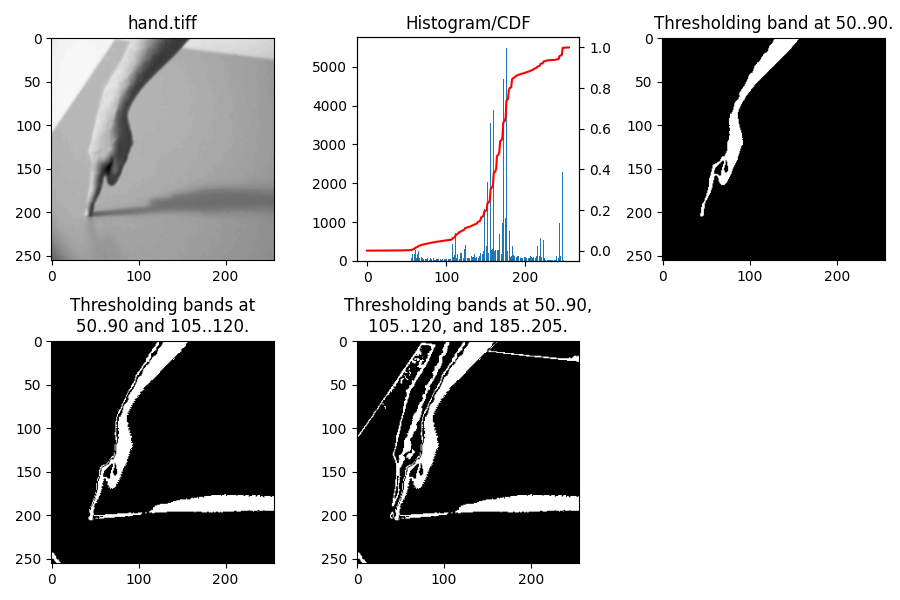
\includegraphics[width=\textwidth]{figures/task_5_1_example1.png}
  \caption{\texttt{hand.tiff} -- example illustrating problem \#1.}
  \label{fig:hand}
\end{figure}


\paragraph{Problem \#2:} intensity-based segmentation can run into trouble with
noise in images, since (white) noise is likely to appear in the histogram as
foreground object pixels due to the high intensity pixels.
\Cref{fig:5_1_example2} shows an example of this. In addition, noise
which appears in multiple different intensities can obscure the ``valleys'' in
the histogram, making it (especially) difficult to determine thresholding
values/bands.

\begin{figure}[H]
  \centering
  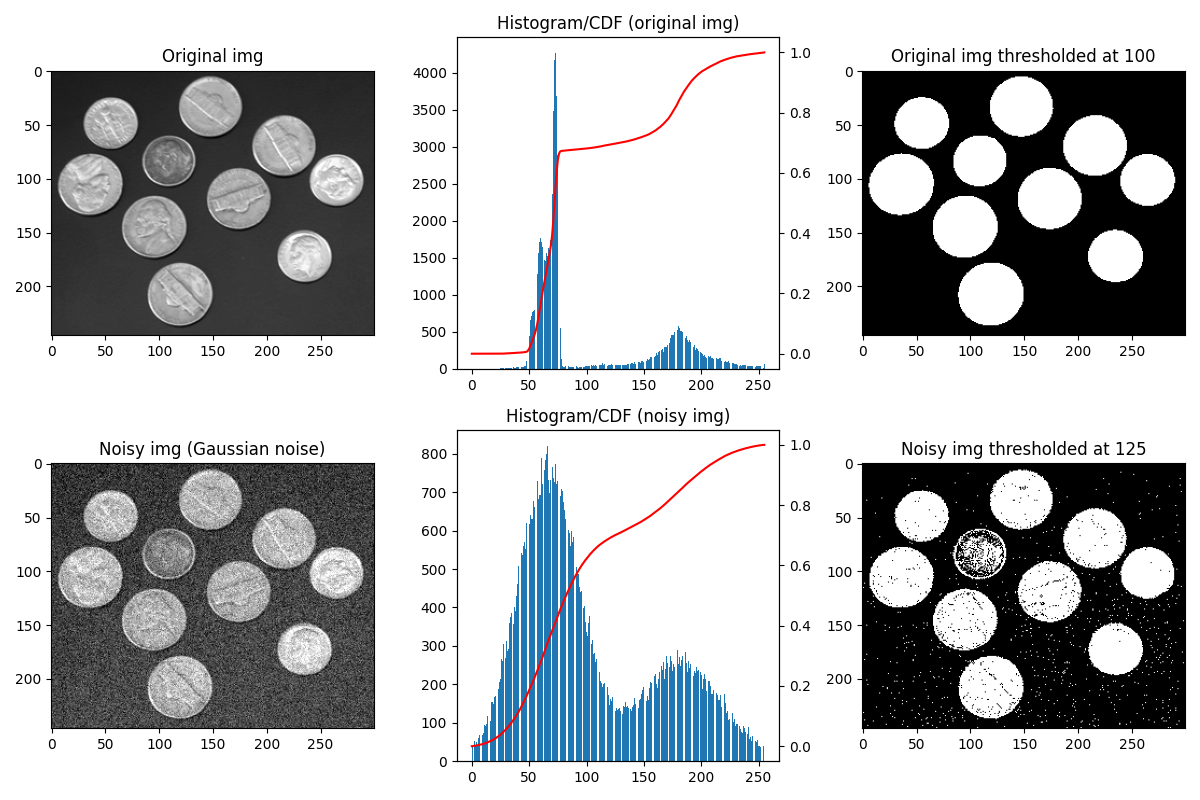
\includegraphics[width=\textwidth]{figures/task_5_1_example2.png}
  \caption{Threshold segmentation of \texttt{coins.png} with and without
  Gaussian noise -- example of problem \#2.}
  \label{fig:5_1_example2}
\end{figure}


\paragraph{Problem \#3} is segmentation tasks with multiple objects in
different intensities and the manual work usually associated with them. In these
cases we might see a necessity for multiple thresholding bands since a single
catch-all threshold value that works for all foreground objects might accept
unwanted parts of the background. Adding additional thresholding bands is in
itself not hard, but it can be very tedious process and can eliminate the
benefits of automatic segmentation.

Whenever we add a separate thresholding band, we add another dimension to the
parameter search for the optimal thresholding values, and each time we add a
thresholding band we possibly let some of the background bleed through (similar
to what we saw in \cref{fig:hand}).

\subsection{Edge-based vs intensity-based segmentation}

First of all, edge-based segmentation can in most cases solve problems \#1 and
\#, since edge-based segmentation is (to some degree) ignorant of similarity
between pixels inside a foreground object and the background, so long as there
is a clearly defined edge surrounding the object. In \cref{fig:hand} we saw how
the soft color gradient on the arm/hand in the x-direction caused trouble for
thresholding, but since there are clearly defined edge between the arm and
background, edge-based segmentation might succeed here. A similar thing goes for
multiple foreground objects in different intensities, so long as they have
clearly defined edges.

With respect to noisy images, edge-based segmentation has its own problems,
since noise can obscure edges and even create spurious ``extra'' edges.

An example of where edge-based segmentation might perform badly are cases where
the background itself has sharp edges, such as a tiled floor, and if the back-
and foreground object happen to be clearly distinguished in intensity, then
thresholding might give an even better result than edge-based.
